\section{$\Theta$ Sketch}
\label{sec:theta}


We have given an overview the sequential sketch in Section~\ref{subsubsec:theta-sketch}, 
and shown the composable sketch implementation in Section~\ref{subsubsec:composable-Theta-sketch}.
Section~\ref{ssec:theta-analysis} analyses the algorithm's correctness and error bounds.

\subsection{Error bounds}
\label{ssec:theta-analysis}
We analyse the error introduced by an $r$-relaxation $SeqSketch^r$ of the $\Theta$ sketch.
Given Lemma~\ref{lemma:genereic-strong} above, the concurrent sketch's error is bounded
by the relaxation's error bound for $r=2N$$b$.

Consider a set of $n$ labelled random variables $A_1,\dots,A_n$, which our hash function
maps to the interval $[0,1]$. Let $M_{(i)}$ be the $i^th$ minimum value. The adversary
chooses up to $r$ variables to hide from the query.

Consider first a strong adversary, who knows the oracle's coin flips. Let $est(i)=\frac{k-1}{M_{(i)}}$
be the estimate returned by the query if $\Theta = M_{(i)}$. The strong adversary chooses the
estimate that maximises the error of the query. The value of $\Theta$ is the maximum value in the maxheap
of size $k$, so $\Theta$ is chosen out of the collection $\Set{M_{(k+j)}}{0 \leq j \leq r}$.
The adversary will hide $r$ updates such that $\Theta = M_{(k)}$ or $\Theta = M_{(k+r)}$. This is because
$M_{(k)} \leq M_{(k+1)} \leq \dots \leq M_{(k+r)}$, so the choice that maximises the error is at the edges.
Therefore, if $W$ is the estimate the strong adversary ``forces'', then:
\[
W(est(k), est(k+r)) = \begin{dcases*}
    est(k) & $\abs{est(k) - n} > \abs{est(k+r) - n}$ \\
    est(k+r) & else
    \end{dcases*}
\]

In Figure~\ref{fig:areaGraph} we show the plot of $M_{(k)}$ and $M_{(k+r)}$, with the lines for when
$\abs{est(k) - n} = \abs{est(k+r) - n}$. In the blue area $M_{(k+r)} < M_{(k)}$, and in
the orange area $M_{(k)} < M_{(k+r)}$.
\begin{figure}[H]
    \centering
    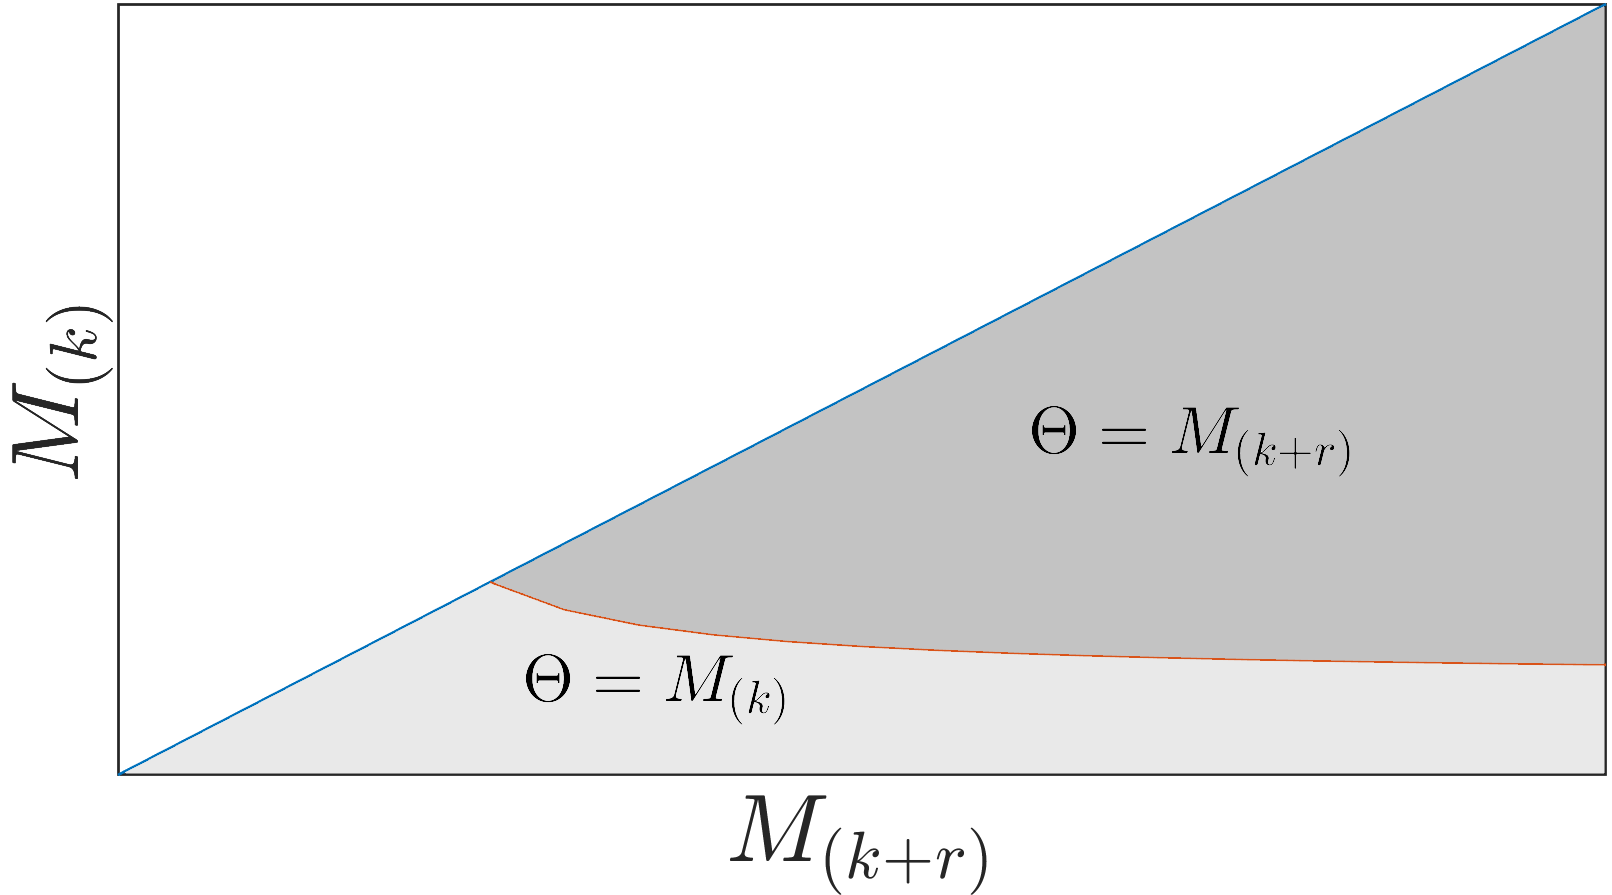
\includegraphics[width=6in]{images/areaGraph.png}
    \caption{Graph of joint probability areas.}
    \label{fig:areaGraph}
\end{figure}
\begin{figure}[H]
    \centering
    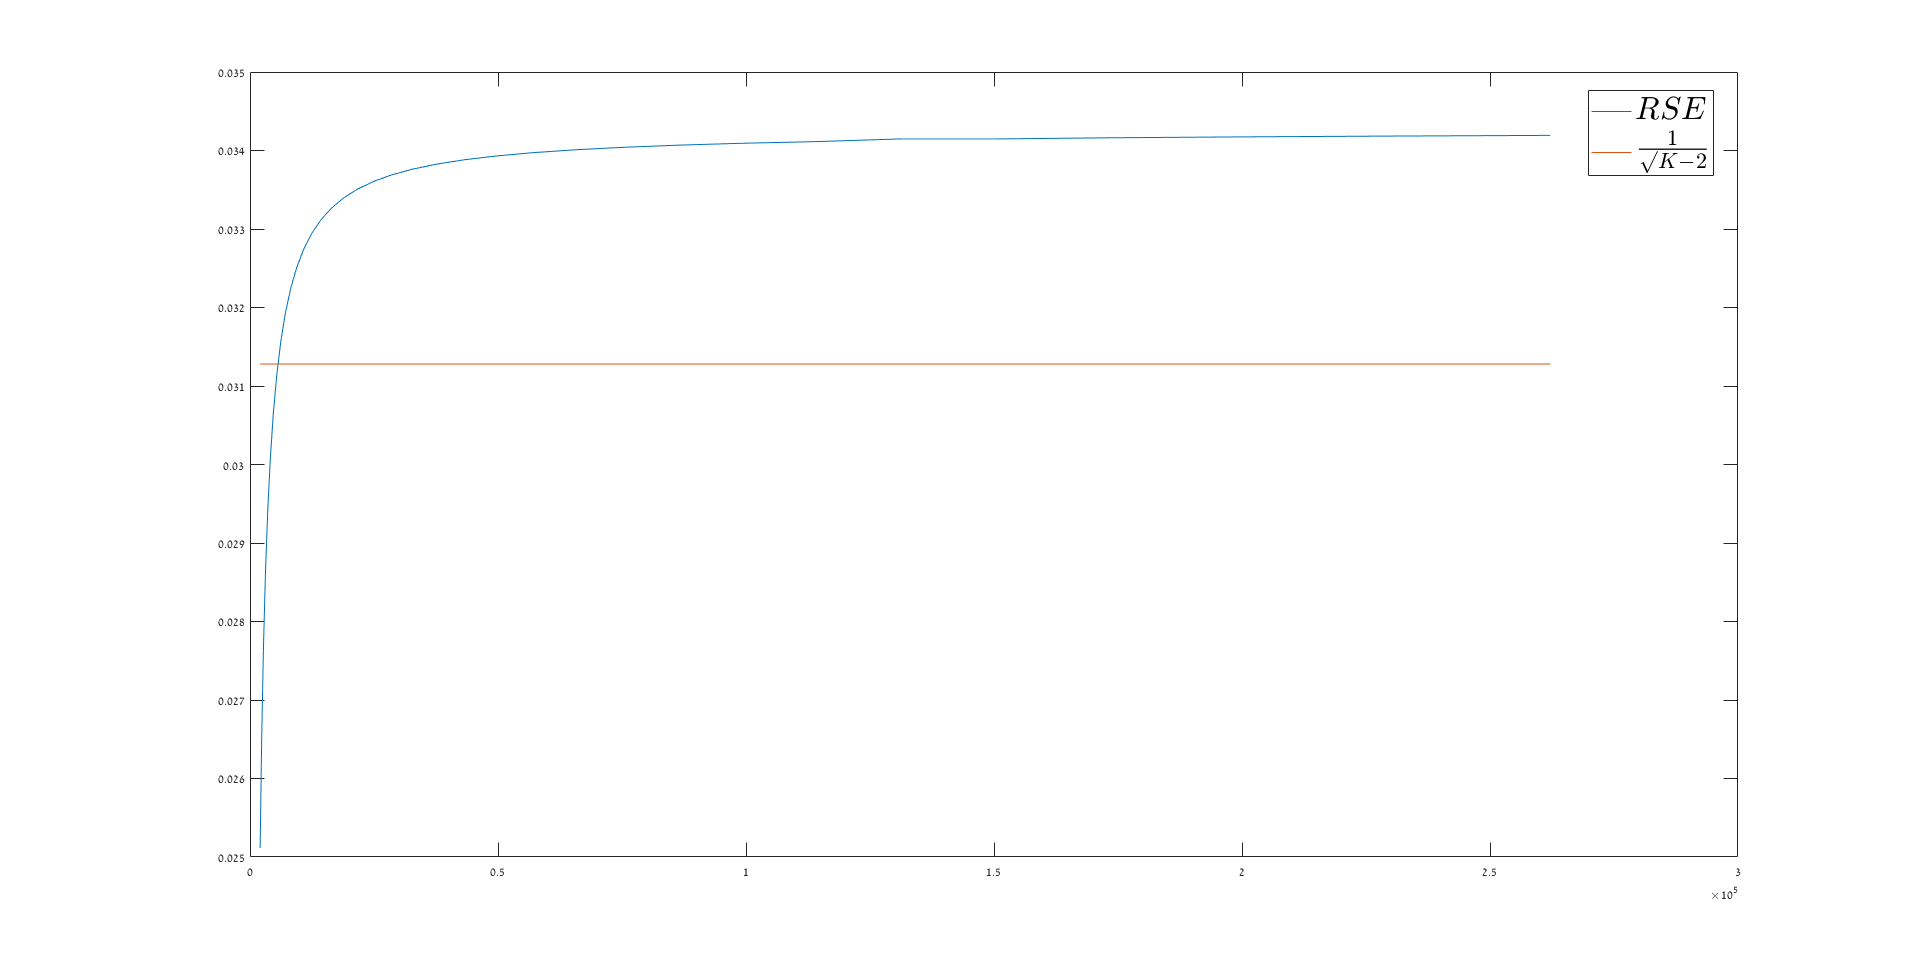
\includegraphics[width=6in]{images/strongAdversaryRSE.png}
    \caption{RSE of $W$.}
    \label{fig:strongAdversaryRSE}
\end{figure}

We would like to know what the $RSE$ of $W$ is. If can be shown that for the order statistics 
$M_{(k)}, M_{(k+r)}$, the join probability density function is:
\begin{align*}
f_{M_{(k)},M_{(k+r)}}(m_k,m_{k+r}) = n!{m_k^{k-1}\over (k-1)!}{(m_{k+r}-m_k)^{r-1}\over(r-1)!}{(1-m_{k+r})^{n-(k+r)}\over (n-(k+r))!}.
\end{align*}

We show the numerical solution \footnote{We conjecture that this integral is nonelementary.}
in Figure~\ref{fig:strongAdversaryRSE} for the RSE introduced by the strong adversary,
for $r=8,K=1024$. The results show that the strong adversary increases the RSE by $0.3\%$. Given
that for $K=1024$ the RSE of the sequential sketch is $3.1\%$, the increase is negligible.

We note that $est(k+r)<est(k)$, therefore if $est(k)<n$ the adversary will choose $est(k+r)$.
\begin{align*}
    P(est(k)<n)=P\left({k-1 \over M_{(k)}}<n\right)=P\left({k-1 \over n}<M_{(k)}\right)=\left(1-\frac{k-1}{n}\right)^{k+1}
\end{align*}
When $n\rightarrow\infty$ then $P(est(k) \leq n) \rightarrow 1$, therefore the most likely choice is for the strong
adversary to choose $est(k+r)$. Given $K=1024$ and $n=10^4(k-1)$, we get that $P(est(k)<n) > 0.9$.

Now, consider a weaker adversary. This adversary always hides the $r$ smallest elements, 
thereby ``choosing'' $est(k+r)$. In this case we use order statistics to calculate the exact.
From order statistics, the expected estimate of the sketch is:
\begin{align*}
    E[est(k+r)]=E\left[ \frac{K-1}{M_{(k+r)}} \right]=n\frac{k-1}{k+r-1}   
\end{align*}
The variance of $est(k+r)$:
\begin{align*}
    \sigma^2[est(k+r)] = E[est(k+r)^2] - E[est(k+r)]^2
\end{align*}
Returning the evaluation of $E[est(k+r)^2]$:
\begin{align*}
    E[est(k+r)^2]=(k-1)^2\frac{n(n-1)}{(k+r-1)(k+r-1)}
\end{align*}
We plug all this into the variance to get:
\begin{align*}
    \sigma^2[est(k+r)] &= E[est(k+r)^2] - E[est(k+r)]^2 \\
    &=(k-1)^2\frac{n(n-1)}{(k+r-1)(k+r-1)} - \left(n\frac{k-1}{k+r-1} \right)^2 \\
    &=\frac{n(k-1)^2}{k+r-1}\left[\frac{n-1}{k+r-2}-\frac{n}{k+r-1}\right] \\
    &=\frac{n(k-1)^2}{k+r-1}\left[\frac{n(k+r-1)-(k+r-1)-n(k+r-1)+n}{(k+r-2)(k+r-1)}\right] \\
    &=\frac{n(k-1)^2}{k+r-1}\left[\frac{n-(k+r-1)}{(k+r-2)(k+r-1)}\right] \\
    &< \frac{n(k-1)^2}{k+r-1}\left[\frac{n}{(k+r-2)(k+r-1)}\right] \\
    &=\frac{n^2(k-1)^2}{(k+r-2)(k+r-1)^2} < \frac{n^2}{k+r-2} \\
    \sigma^2[est(k+r)] &< \frac{n^2}{k+r-2}
\end{align*}

Normalizing the variance by $n^2$ and taking the square root results in the RSE:
\begin{align*} 
    RSE[est(k+r)]=\sqrt{{\sigma^2[est(k+r)]\over n^2}}<\sqrt{{\frac{n^2}{k+r-2} \over n^2}}=\sqrt{\frac{1}{k+r-2}}
\end{align*}

In the case where $k \gg r$, $RSE[est(k+r)]$ is almost the same as the RSE of the sequential $\Theta$ sketch,
and the estimate returned by the sketch is is almost the same as the estimate of the sequential $\Theta$ sketch.